\documentclass[10pt,conference]{IEEEtran}

\usepackage[utf8]{inputenc}
\usepackage{graphicx}
\usepackage{url}
\usepackage{enumitem}
\usepackage{float}
\usepackage{fvextra}


\title{3rd Lab with VTK (Visualization Tool Kit)}

\author{
\IEEEauthorblockN{João Varela, 113780}
\IEEEauthorblockN{Carolina Prata, 114246}
\IEEEauthorblockA{Information Visualization, 2025\\
MSc in Computer Engineering, University of Aveiro}
}

\begin{document}

\maketitle

\begin{abstract}
This document provides a brief description of the work developed for the third lab of the Information Visualization course, with the objective of understanding how glyphing, picking, unstructured grids, and the association of scalars with vectors and grids work.
\end{abstract}

\section{Introduction}
The Visualization Toolkit (VTK) is an open-source software framework extensively used in 3D computer graphics, image processing, and scientific visualization, offering robust tools for handling a wide range of data types and supporting visualization methods such as volume rendering, contouring, and streamline analysis. In addition to features such as multiple actors and renderers, shading options, textures, transformations, and observers with callbacks, VTK also provides mechanisms for glyphing, picking, unstructured grid representations, and the association of scalar data with vectors and grids.

\section{Development}

The laboratory assignment provided by the course instructor comprises several exercises covering the following topics:

\begin{itemize}
    \item Glyphing;
    \item Picking;
    \item Unstructured Grid;
    \item Scalar association to vectors and grids;
    \item HedgeHog;
\end{itemize}


\subsection{Glyphing}
For the first exercise, we explored the \texttt{vtkGlyph3D} class to understand the concept of glyphing and how data can be represented using geometric symbols. The objective was to visualize a sphere with cones placed at each vertex of the sphere's polygonal mesh, using the cones as glyphs oriented along the surface normals.

To achieve this, a sphere was generated using \texttt{vtkSphereSource} with theta and phi resolutions of 30, providing the input dataset of points where glyphs would be placed on file \texttt{glyph.py}. A cone was created using \texttt{vtkConeSource} to serve as the glyph source the geometric symbol to be replicated at each sphere vertex. The glyphing process was implemented by creating a \texttt{vtkGlyph3D} object and establishing the appropriate connections:

{\small
\begin{Verbatim}[breaklines, breakanywhere]
glyph = vtkGlyph3D()
glyph.SetSourceConnection(coneSource.GetOutputPort())
glyph.SetInputConnection(sphereSource.GetOutputPort())
glyph.SetScaleFactor(0.25)
glyph.SetVectorModeToUseNormal()
\end{Verbatim}
}
The \texttt{SetScaleFactor} method scales the cones to 25\% of their original size, ensuring appropriate proportions relative to the sphere's surface. The \texttt{SetVectorModeToUseNormal} method orients each glyph according to the normal vectors at the sphere's vertices, causing all cones to point radially outward, perpendicular to the surface.

Experimenting with different theta and phi resolution values using \texttt{SetThetaResolution} and \texttt{SetPhiResolution} reveals significant differences in glyph distribution. Lower resolutions (e.g., 10) produce fewer vertices and thus fewer, more sparsely distributed glyphs, while higher resolutions (e.g., 50) generate a denser mesh with more glyphs, creating a smoother and more detailed representation of the sphere's surface structure.

\begin{figure}[H]
\centering

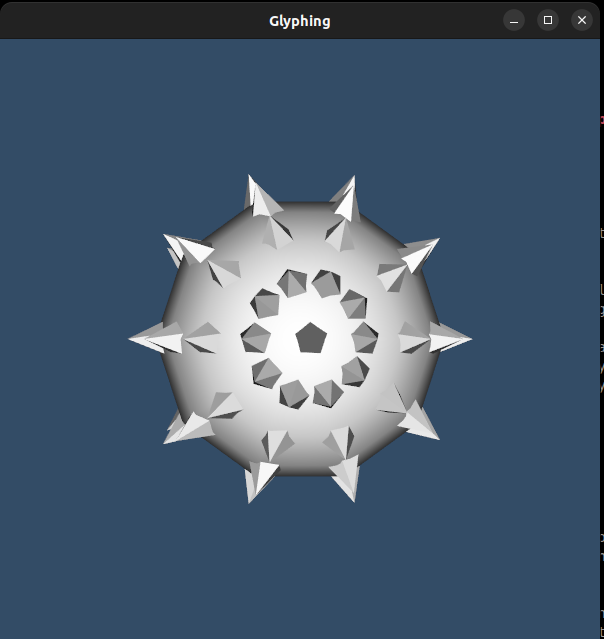
\includegraphics[width=0.20\textwidth]{lesson3/10.png}
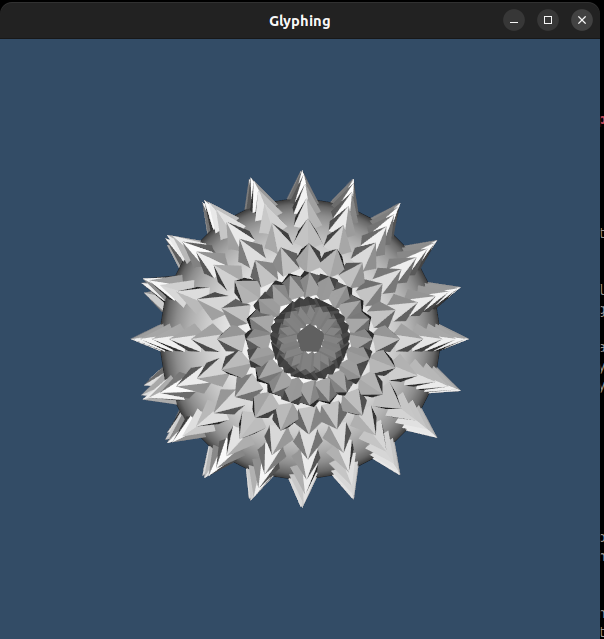
\includegraphics[width=0.20\textwidth]{lesson3/20.png}

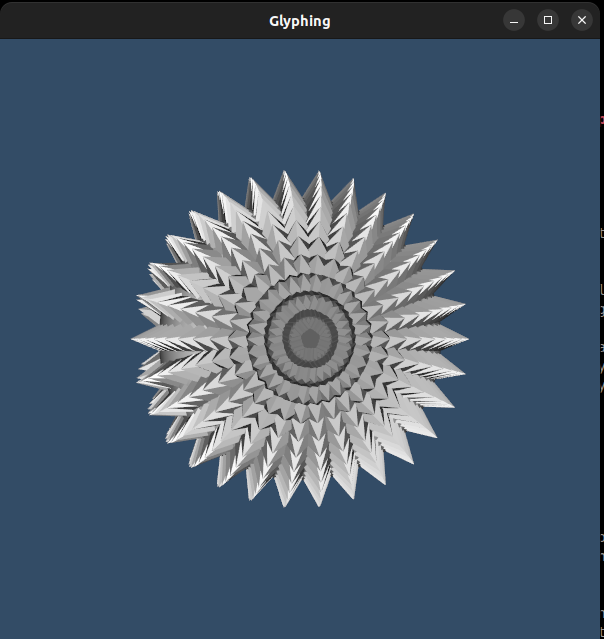
\includegraphics[width=0.20\textwidth]{lesson3/30.png}
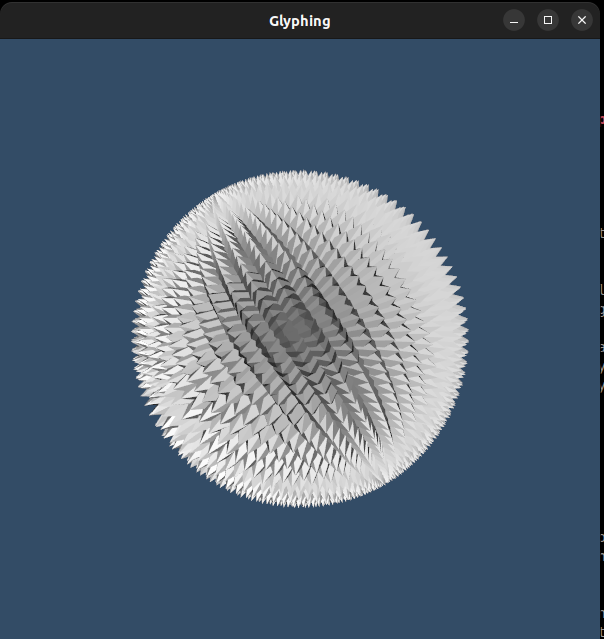
\includegraphics[width=0.20\textwidth]{lesson3/50.png}

\caption{ Results obtained by executing the first exercise with different values for the Scale Factor, Theta, and Phi resolution, using 10, 20, 30, and 50, respectively.}
\end{figure}


\subsection{Picking}

In this exercise, in file \texttt{pick.sample}, a point picking mechanism was added to the interactor of the previous example in order to enable the selection of points on the rendered model. This functionality allows the user to interactively identify specific positions on the surface during execution.

To visually represent the selected point, an additional sphere actor was created. Its visibility was initially disabled using \texttt{VisibilityOff()}, ensuring that it would only become visible when a pick event occurs. A callback class was then implemented to handle the picking event and update the scene accordingly:
\setlength{\intextsep}{6pt}
{\small
\begin{Verbatim}[breaklines, breakanywhere]
def __init__(self, picker, sphere_actor, render_window):
    self.picker = picker
    self.sphere_actor = sphere_actor
    self.render_window = render_window

def __call__(self, obj, event):
    pickPosition = self.picker.GetPickPosition()
    print(f"Picked point coordinates: {pickPosition}")
    
    self.sphere_actor.SetPosition(pickPosition)
    self.sphere_actor.VisibilityOn()
    self.sphere_actor.GetProperty().SetColor(1.0, 0.0, 0.0)
    self.render_window.Render()
\end{Verbatim}
}


This callback class is responsible for handling the pick event. When a point is selected, the \texttt{\_\_call\_\_} method retrieves the coordinates of the picked position using \texttt{GetPickPosition()}. The sphere actor is then moved to the selected location, its visibility is enabled, and its color is set to red in order to clearly highlight the picked point. The render window is subsequently updated to reflect these changes. Additionally, the picked coordinates are printed to the terminal for verification purposes.

The picking mechanism was configured by creating an instance of \texttt{vtkPointPicker}, referred to as \texttt{myPicker}. The callback was instantiated as \texttt{mo1 = vtkMyCallback(myPicker, selectedSphereActor, renderWindow)} and registered with the picker using \texttt{AddObserver(vtkCommand.EndPickEvent, mo1)}. Finally, the picker was associated with the interactor through \texttt{iren.SetPicker(myPicker)}. 
The picking action is triggered during interaction by pressing the \texttt{P} key.

\setlength{\intextsep}{6pt}
\begin{figure}[H]
\centering
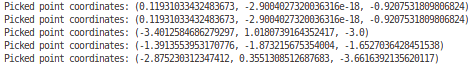
\includegraphics[width=1\columnwidth]{lesson3/terminal_prints.png}
\end{figure}

\begin{figure}[H]
\centering
\begin{minipage}{0.45\columnwidth}
    \centering
    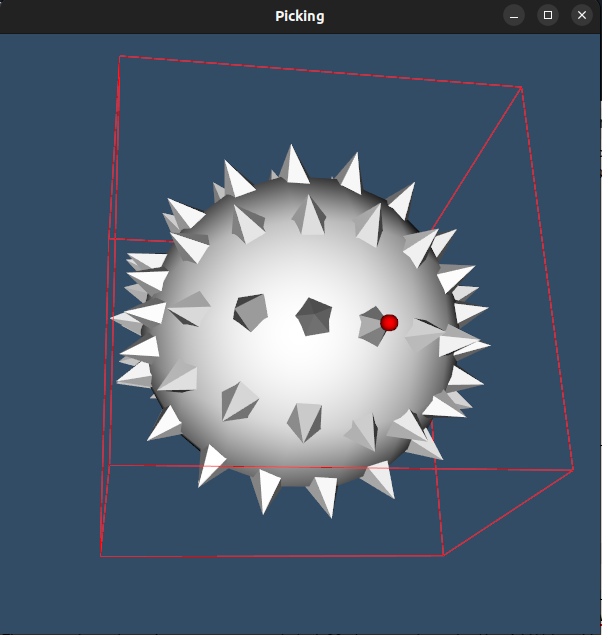
\includegraphics[width=\linewidth]{lesson3/pick_esfera.png}
\end{minipage}
\hfill
\begin{minipage}{0.45\columnwidth}
    \centering
    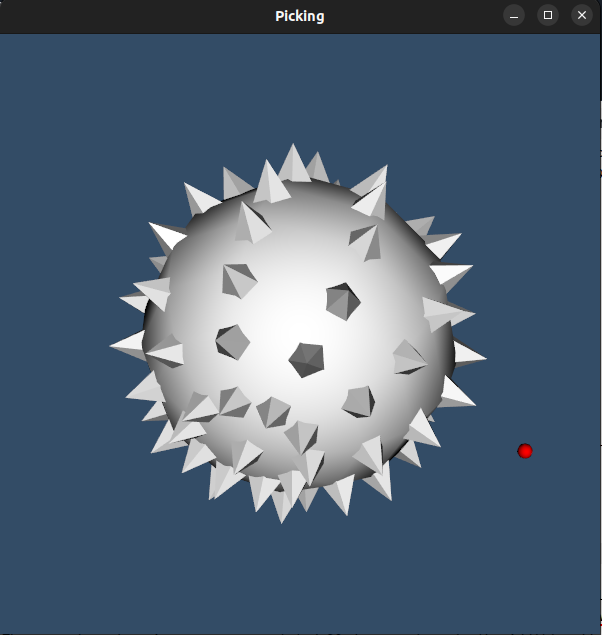
\includegraphics[width=\linewidth]{lesson3/pick_fora.png}
\end{minipage}
\caption{Result of the execution of the second exercise)}
\end{figure}


\subsection{Display Coordinates}
As an extension to the object picking exercise, an additional task was implemented in which the picked point coordinates are displayed directly within the renderer window, rather than being printed to the terminal. To achieve this, a text visualization mechanism was introduced using a \texttt{vtkTextMapper} combined with a 2D actor, enabling the coordinates of the selected point to be rendered on screen, in \texttt{coordinates.py}.

Similarly to the previously used sphere actor, the text actor was initially created with its visibility set to off, ensuring that no text is displayed until a point picking event occurs. When such an event is triggered, the callback function is updated to convert the picked position into a formatted string representing the $(x, y, z)$ coordinates with two decimal places. The text mapper is then updated with this information, the text actor is made visible, and its position is adjusted with a small offset relative to the picked point to improve readability. Finally, the render window is updated to reflect these changes.

\begin{figure}[H]
\centering
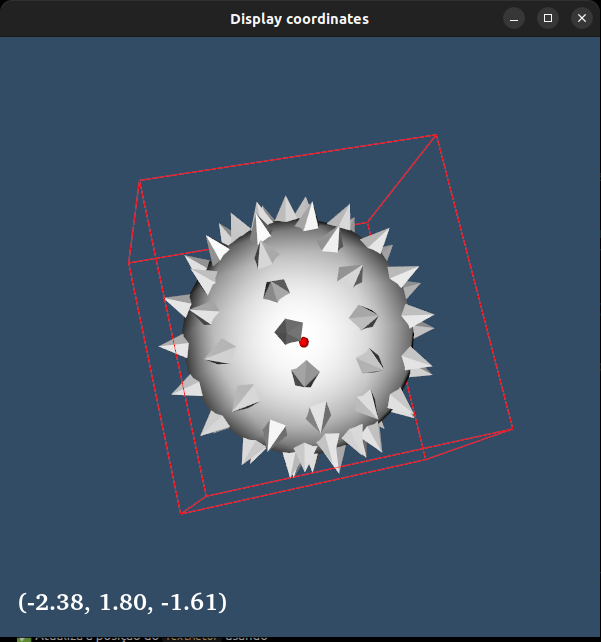
\includegraphics[width=0.40\textwidth]{lesson3/display.png}
\caption{Point picking visualization displaying selected coordinates in the render window}
\end{figure}

\subsection{Unstructured Grid}
For this exercise, a source file was provided containing code that makes use of VTK’s \texttt{vtkUnstructuredGrid}. The implementation constructs an unstructured grid composed of a single cell, specifically a tetrahedron. Upon executing the file, the following result was obtained:

\begin{figure}[H]
\centering
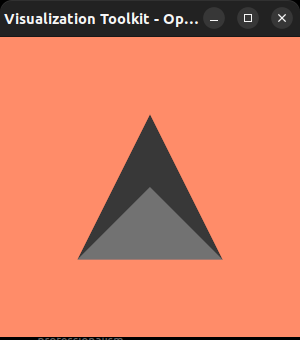
\includegraphics[width=0.30\textwidth]{lesson3/ugrid_default.png}
\caption{Result of the execution of the file \texttt{ugrid.py} provided by the
professor}
\end{figure}

In this exercise, the initial implementation displaying a tetrahedral cell (\texttt{VTK\_TETRA}) was modified so that each vertex is represented as an independent cell using \texttt{VTK\_VERTEX}. Instead of a single tetrahedron composed of four connected vertices, individual vertex cells were created, treating each point as a separate entity within the unstructured grid.

This was achieved by iterating over the list of point coordinates and, for each coordinate, creating a corresponding \texttt{VTK\_VERTEX} cell. Additionally, the visual properties of the actor were adjusted by setting its color to red and increasing the point size to five, thereby improving the visibility of the individual vertices. The renderer background color was also changed to a light gray in order to enhance contrast.

As a result of these modifications, the visualization displays clearly defined red points, rather than a connected tetrahedral structure.

\begin{figure}[H]
\centering
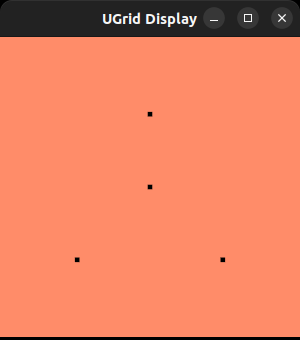
\includegraphics[width=0.30\textwidth]{lesson3/ugrid_final.png}
\caption{ Results obtained by executing the \texttt{ugrid.py} file after changes}
\end{figure}

\subsection{Scalar association to vectors and grids}
In this section, the exercise focused on the creation of an unstructured grid composed of four points, with each point associated with both a vector and a scalar value. The vector data, defined as $(1,0,0)$, $(0,1,0)$, $(0,0,1)$, and $(1,1,1)$, were stored in a \texttt{vtkFloatArray} with three components and used to define the orientation of the glyphs. These vectors were subsequently applied to orient cone glyphs positioned at each grid point using the \texttt{vtkGlyph3D} class.

In addition to the vector data, scalar values $(0.1, 0.3, 0.5, 0.8)$ were assigned to the corresponding points and stored in a separate \texttt{vtkFloatArray}. These scalar values were employed to control the coloring of the cones, enabling a visual representation of scalar variation across the grid.

The implementation begins by creating an unstructured grid and inserting the four points as individual \texttt {VTK\_VERTEX} cells. The vector and scalar arrays are then defined and associated with the grid points. A \texttt{vtkGlyph3D} object is used to generate cone glyphs at each point, with their orientation driven by the vector data and their appearance influenced by the associated scalar values. The resulting visualization is rendered against a light gray background, as shown below.

\begin{figure}[H]
\centering
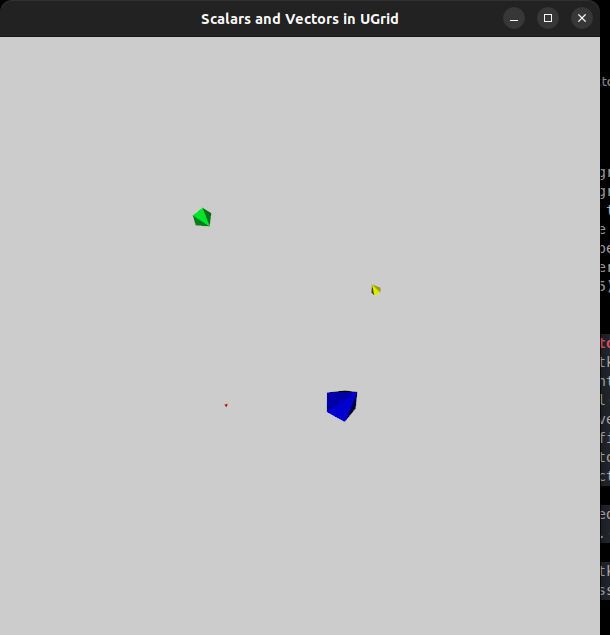
\includegraphics[width=0.40\textwidth]{lesson3/scalar.png}
\caption{ Results obtained by executing the \texttt{scalar.py} file}
\end{figure}

\subsection{HedgeHog}
In the final exercise, the visualization of vector data was explored using the \texttt{vtkHedgeHog} class. In contrast to the previous exercise, where vectors were represented using cone glyphs, \texttt{vtkHedgeHog} depicts vector data as line segments, providing a simpler and more direct representation of vector direction and magnitude.

To accomplish this task, the implementation from the previous exercise was adapted by replacing the \texttt{vtkGlyph3D} class with \texttt{vtkHedgeHog}. The hedgehog object was configured to use the vector data associated with the unstructured grid and scaled with a factor of 0.3 in order to control the length of the resulting line segments. The outcome of this modification is illustrated by the visualization obtained below.

\begin{figure}[H]
\centering
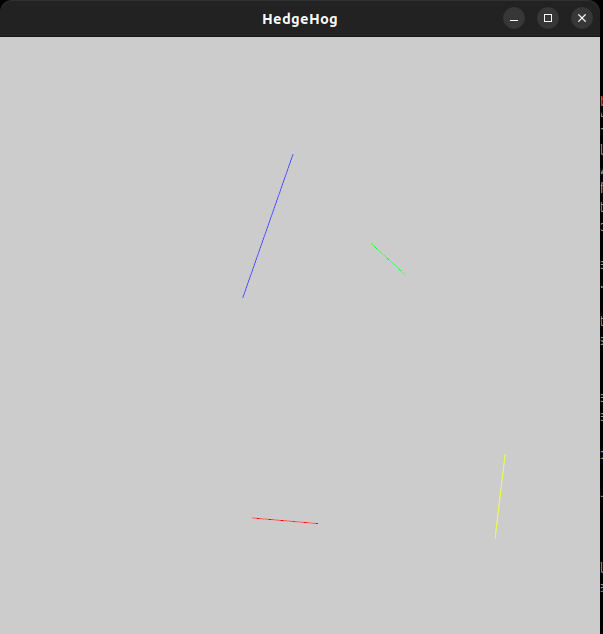
\includegraphics[width=0.40\textwidth]{lesson3/hedge.png}
\caption{ Results obtained by executing the \texttt{hedge.py} file}
\end{figure}

\end{document}
